\pagestyle{fancy}
\fancyhead{} % clear all header fields
\fancyhead[LO,CE]{Tests et validation}
\fancyhead[RO,LE]{2024-2025}
\chapter{Tests et validation}
\section{Application mobile}

\subsection{La page d'accueil}
La figure~\ref{fig:interface-accueil} montre la page d'accueil de l'application. Cette interface permet à l’utilisateur de déclencher une distribution manuelle et de visualiser le distributeur sélectionné, la quantité de ration actuelle, ainsi que les alertes causées par le seuil critique configuré.\\

\begin{minipage}{\linewidth}
  \centering
  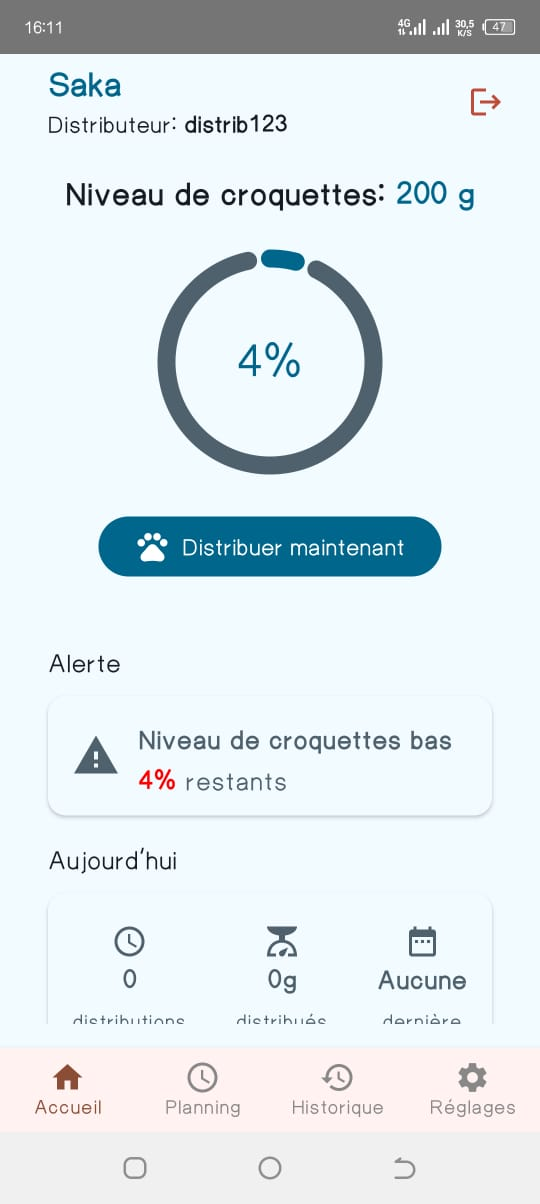
\includegraphics[scale=0.25]{page-acceuil.jpeg}
  \captionof{figure}{Interface d'accueil de l'application mobile}
  \label{fig:interface-accueil}
\end{minipage}

\subsection{Planning de Distribution}
La figure~\ref{fig:interface-planning} montre la page de planification. Elle permet à l'utilisateur de voir les prochaines distributions prévues. Il peut activer ou désactiver les heures de distribution, mettre temporairement en pause toutes les distributions, ou reprendre manuellement le fonctionnement. Un indicateur affiche aussi l’état de connexion du distributeur.\\

\begin{minipage}{\linewidth}
  \centering
  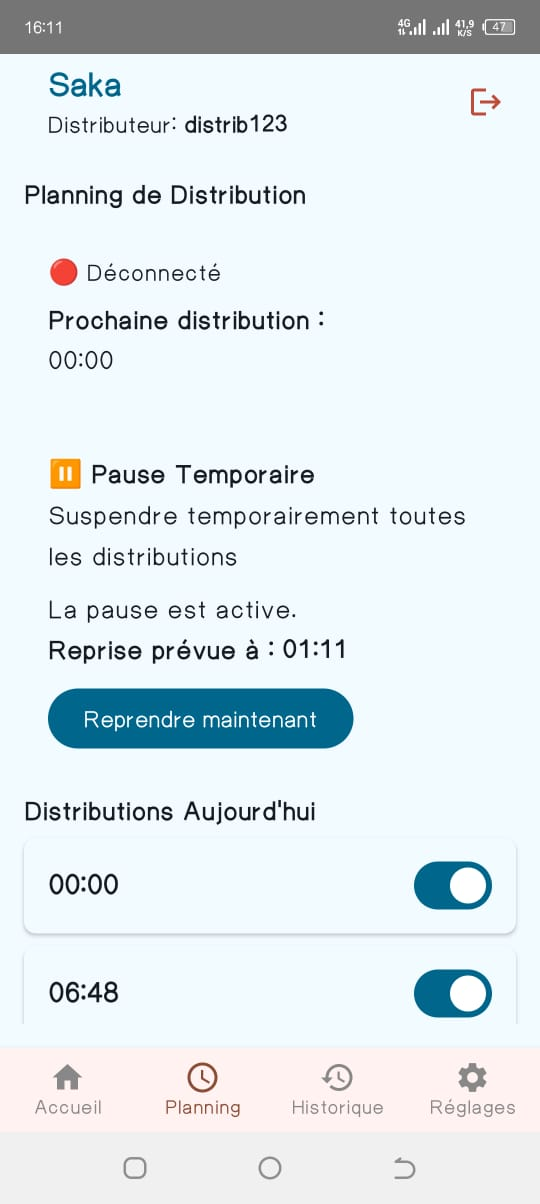
\includegraphics[scale=0.25]{page-planning.jpeg}
  \captionof{figure}{Page de planification des distributions}
  \label{fig:interface-planning}
\end{minipage}

\subsection{Liste des historiques}
La figure~\ref{fig:interface-historique} montre la page d’historique. Elle affiche toutes les distributions de nourriture effectuées, avec l’heure, la date, la quantité distribuée et le statut de réussite. L’utilisateur peut consulter donc l’historique d’aujourd’hui ou de toute la semaine.\\

\begin{minipage}{\linewidth}
  \centering
  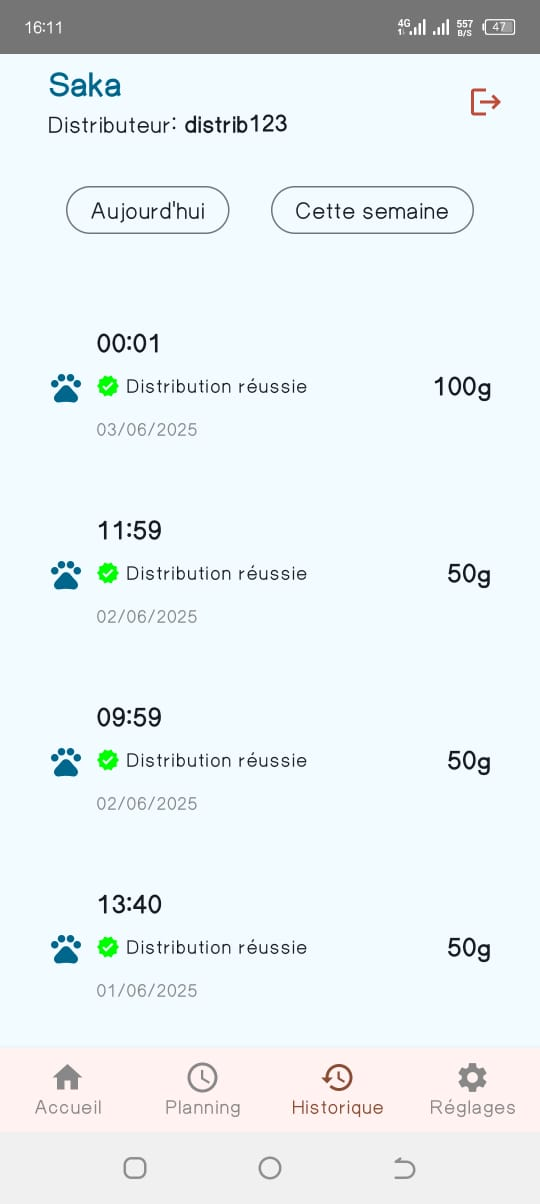
\includegraphics[scale=0.25]{page-historique.jpeg}
  \captionof{figure}{Historique des distributions de nourriture}
  \label{fig:interface-historique}
\end{minipage}

\subsection{Interface de réglages}
Cette section de l’application, illustré dans la figure~\ref{fig:interface-reglage}, permet à l’utilisateur de configurer des paramètres comme la quantité de ration à distribuer ou le seuil critique. Les champs de saisie permettent d’entrer ces valeurs manuellement, puis de les valider. Ces options donnent plus de contrôle à l'utilisateur sur la gestion de la distribution de nourriture.\\

\begin{minipage}{\linewidth}
  \centering
  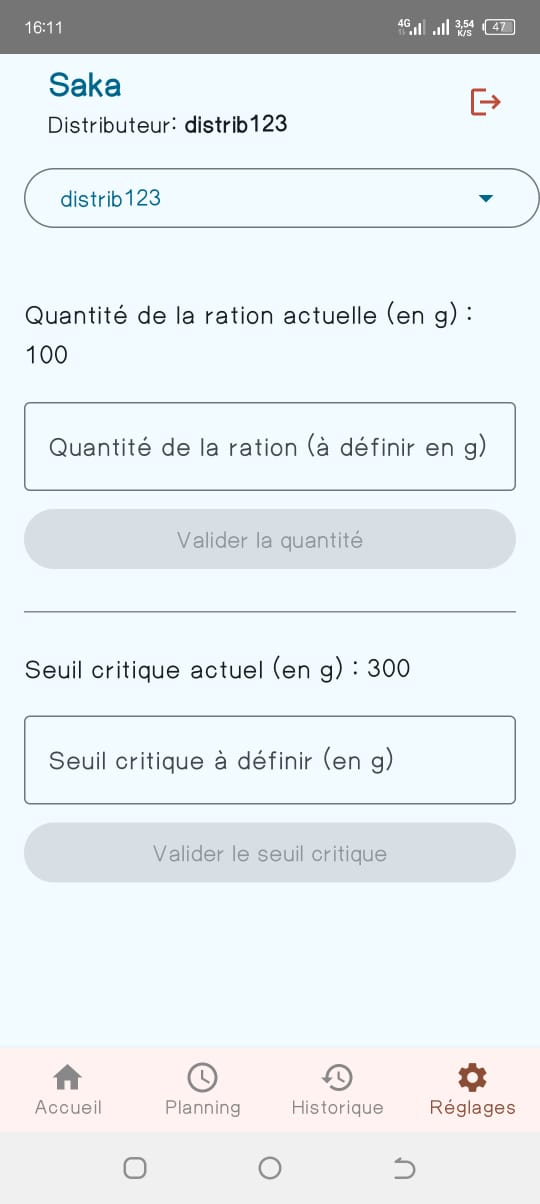
\includegraphics[scale=0.25]{page-reglage.jpeg}
  \captionof{figure}{Historique des distributions de nourriture}
  \label{fig:interface-reglage}
\end{minipage}

\section{Distributeur automatique}

Pour tester le fonctionnement du système, et comme il n'est pas possible de montrer directement le matériel ici, nous utilisons l' \verb|interface série (Serial)| de l'ESP32 pour vérifier que le code de distribution s'exécute correctement.

\subsection{Distribution manuelle et automatique}

Dans la figure~\ref{fig:message-websocket}, lorsque le message reçu est de type \verb|"t"|, cela déclenche une distribution manuelle. Le message "Trigger food" s'affiche alors dans le \verb|Serial monitor|. Cela montre que la commande envoyée depuis l'application mobile a bien été prise en compte. La figure~\ref{fig:trigger-manual} illustre ce processus.\\

\begin{minipage}{\linewidth}
\centering
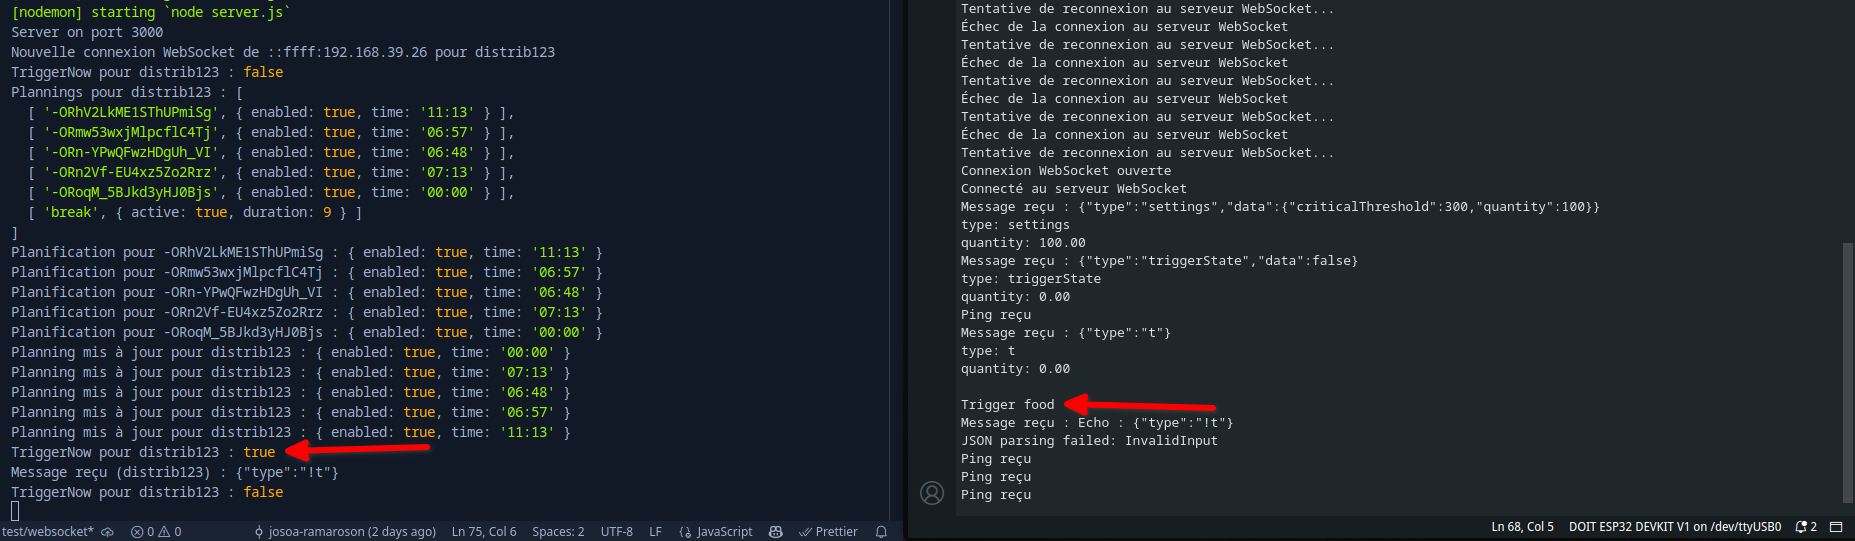
\includegraphics[scale=0.32]{trigger-manual.png}
\captionof{figure}{Message affiché lors d'une distribution manuelle}
\label{fig:trigger-manual}
\end{minipage} \\


Pour une distribution planifiée, le message reçu est de type \verb|"sct"|. Dans ce cas, le texte "Trigger Scheduled food" s'affiche dans le \verb|Serial monitor|, comme illustré dans la figure~\ref{fig:trigger-auto}. Cette action est déclenchée automatiquement selon un planning défini via des scripts Cron, dont l'exécution est aussi visible dans cette figure.\\

\begin{minipage}{\linewidth}
\centering
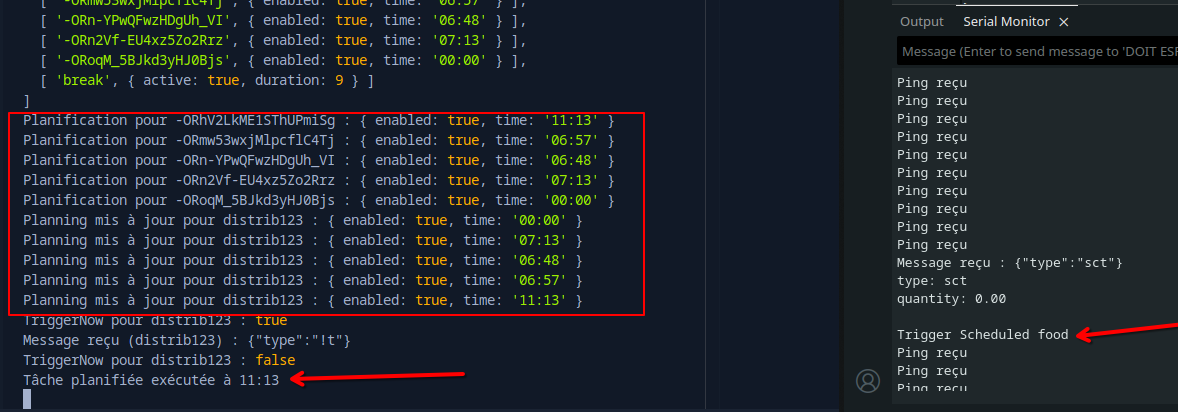
\includegraphics[scale=0.5]{planning-image.png}
\captionof{figure}{Message affiché lors d'une distribution automatique (planifiée)}
\label{fig:trigger-auto}
\end{minipage}

